\documentclass[12pt,a4paper,oneside]{article}
\usepackage[a4paper,left=3cm,right=2cm,top=2.5cm,bottom=2.5cm]{geometry}
\usepackage{graphicx}
\usepackage{lineno}
\usepackage{enumitem} 
\usepackage{lscape}
\usepackage{hyperref} 
\usepackage{apacite}
\usepackage{booktabs}
\usepackage{tikz}
\usepackage{multicol} 
\usetikzlibrary{shapes.geometric, arrows}

\tikzstyle{startstop} = [rectangle, rounded corners, minimum width=1.5cm, minimum height=1cm,text centered, draw=black, fill=red!30]
\tikzstyle{io} = [trapezium, trapezium left angle=70, trapezium right angle=110, minimum width=3cm, minimum height=1cm, text centered, draw=black, fill=blue!30]
\tikzstyle{process} = [rectangle, minimum width=3cm, minimum height=1cm, text centered, draw=black, fill=orange!30]
\tikzstyle{decision} = [diamond, minimum width=3cm, minimum height=1cm, text centered, draw=black, fill=green!30]
\tikzstyle{arrow} = [thick,->,>=stealth]



\begin{document}


\begin{center}


\includegraphics[scale=0.30]{mmu.png}\\
\vspace{1cm}
\Large{\textbf{TPT1201 \\Research Methodology in Computer Science}} \\
\vspace{2.5cm}
\Large{\textbf{ASSIGNMENT 1}} \\
\vspace{1cm}
\Large{\textbf{COVID-19 Outbreak Prediction using Machine Learning Techniques}} \\
\vspace{1cm}
 


\vspace{6.5cm}


\normalsize{Prepared by} \\
\vspace{2.5cm}
\large{\textbf{Member Name 1, Student ID 1, Contact Number 1}} \\ 
\large{\textbf{Member Name 1, Student ID 1, Contact Number 1}} \\ 
\large{\textbf{Member Name 1, Student ID 1, Contact Number 1}} \\ 
 

\end{center}

\thispagestyle{empty}
 
\clearpage 

% ============================================

\section{Flowchart}

Provide a detailed discussion about the process flow. Use a diagram to help in explanation. Provide all necessary investigation about the dataset here...

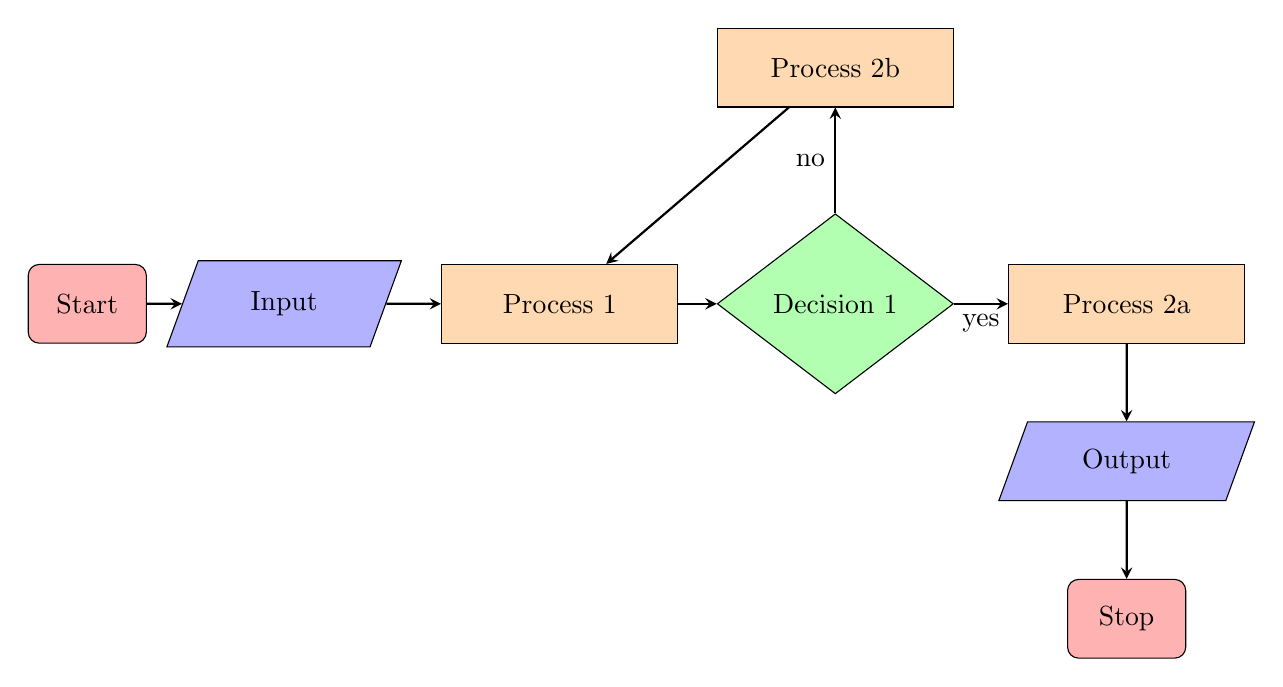
\begin{tikzpicture}[node distance=2cm]
\node (start) [startstop] {Start};
\node (in1) [io, right of=start, xshift=0.5cm] {Input};
\node (pro1) [process, right of=in1, xshift=1.5cm] {Process 1}; 
\node (dec1) [decision, right of=pro1, xshift=1.5cm] {Decision 1};
\node (pro2a) [process, right of=dec1, xshift=1.7cm] {Process 2a};
\node (pro2b) [process, above of=dec1, yshift=1cm] {Process 2b};
\node (out1) [io, below of=pro2a] {Output};
\node (stop) [startstop, below of=out1] {Stop};

\draw [arrow] (start) -- (in1);
\draw [arrow] (in1) -- (pro1);
\draw [arrow] (pro1) -- (dec1); 
\draw [arrow] (dec1) -- node[anchor=north] {yes} (pro2a);
\draw [arrow] (dec1) -- node[anchor=east] {no} (pro2b);
\draw [arrow] (pro2b) -- (pro1);
\draw [arrow] (pro2a) -- (out1);
\draw [arrow] (out1) -- (stop);


\end{tikzpicture}


\section{Insert Table}

In this section, you firstly should discuss why you select a particular model. Why? Answer this first. Then, discuss the performances of models under different settings. You must provide a table for different settings, such as:

\begin{table}[h]
\begin{tabular}{|l|l|}
\hline
Experiment & Parameter Setting          \\ \hline
$\xi1$         & depth = 3, leaf nodes = 10 \\ \hline
$\xi2$          & ...etc                     \\ \hline
$\xi3$         & ...etc                     \\ \hline
\end{tabular}
\end{table}

Provide also a ROC for comparison.
You should add more. Above is just some ideas for your to get things started!

\section{Diagrams}

The models developed has been deployed at http://????
The sample screenshots are given below:

\begin{figure*}[h]
\begin{multicols}{2}
    
\includegraphics[width=\linewidth]{mmu.png}\par 
    
\includegraphics[width=\linewidth]{mmu.png}\par 
    \end{multicols}
\begin{multicols}{2}
    
\includegraphics[width=\linewidth]{mmu.png}\par
    
\includegraphics[width=\linewidth]{mmu.png}\par
\end{multicols}
\caption{Screenshot of Streamlit}
\end{figure*}

\end{document}